\documentclass{beamer}
\usepackage{tikz}

\include{{beamer_header}}

\title{Draw Pictures in \LaTeX}
\subtitle{With \texttt{tikz/pgf}}


\begin{document}

\begin{frame}
  \titlepage
\end{frame}

\begin{frame}{Basic Example}
  \begin{itemize}
    \item The \texttt{pgf/tikz} package allows you to draw pictures from within your \LaTeX{} document.
    \item It enables you to create vector graphics without the need for external tools.
    \item The syntax of \texttt{tikz} involves programming the vector graphics using predefined macros.
  \end{itemize}
\end{frame}

\begin{frame}{A Basic Example}
  \begin{figure}[h!]
    \centering
    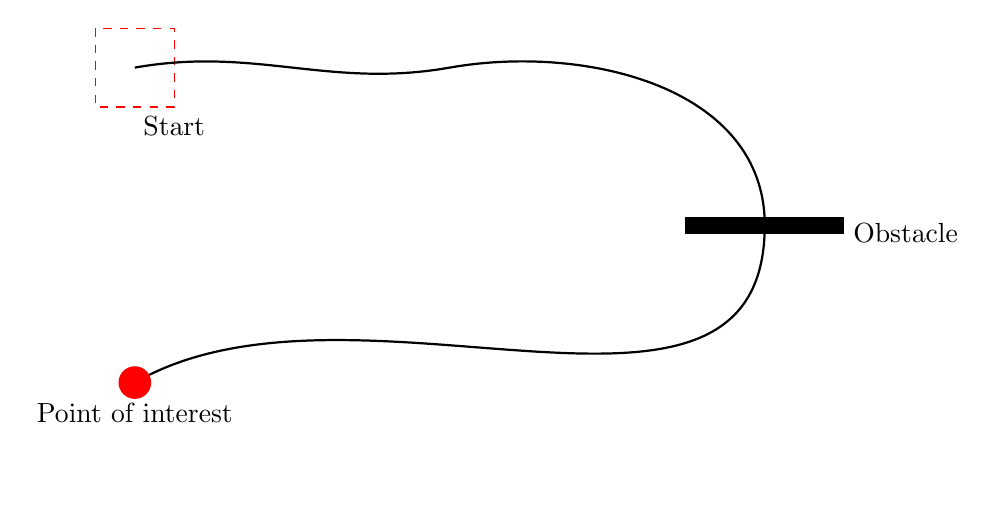
\begin{tikzpicture}
      \draw [red,dashed] (-2.5,2.5) rectangle (-1.5,1.5) node [black,below] {Start};
      \draw [thick] (-2,2) to [out=10,in=190] (2,2) to [out=10,in=90] (6,0) to [out=-90,in=30] (-2,-2);
      \draw [fill] (5,0.1) rectangle (7,-0.1) node [black,right] {Obstacle};
      \draw [red,fill] (-2,-2) circle [radius=0.2] node [black,below=4] {Point of interest};
    \end{tikzpicture}
    \caption{Example graphic made with \texttt{tikz}.}
  \end{figure}
\end{frame}

\begin{frame}{The Syntax of \texttt{tikz}}
  \begin{itemize}
    \item To draw elements with \texttt{tikz}, we use the \texttt{\textbackslash draw} command.
    \item Options for color, line style, etc., can be specified in brackets.
    \item Coordinates are specified in Cartesian coordinates.
    \item Text is placed using \texttt{node} commands.
    \item Each command inside the \texttt{tikzpicture} environment should be terminated with a semicolon.
  \end{itemize}
\end{frame}

\begin{frame}{The Syntax of \texttt{tikz} (contd.)}
  \begin{itemize}
    \item Lines can be drawn by specifying a path using the \texttt{\textbackslash draw} command and the \texttt{to} command.
    \item Bending of lines can be achieved by setting the \texttt{in} and \texttt{out} angles.
    \item There are many more options available for customizing the graphics.
    \item \texttt{tikz} integrates smoothly with the rest of your document.
  \end{itemize}
\end{frame}

\begin{frame}{More Examples}
  \begin{figure}[h!]
    \centering
    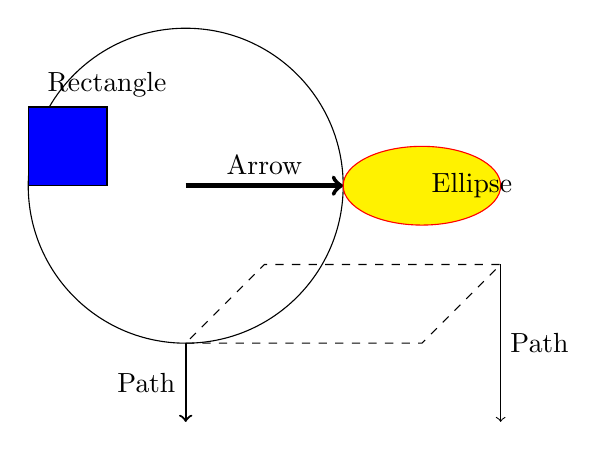
\begin{tikzpicture}
      \draw (0,0) circle [radius=2];
      \draw [fill=blue] (-2,0) rectangle (-1,1) node [black,above] {Rectangle};
      \draw [->,ultra thick] (0,0) -- (2,0) node [black,midway,above] {Arrow};
      \draw [red,fill=yellow] (3,0) ellipse [x radius=1, y radius=0.5] node [black,right] {Ellipse};
      \draw [dashed] (0,-2) -- (3,-2) -- (4,-1) -- (1,-1) -- cycle;
      \draw [->,thick] (0,-2) -- (0,-3) node [black,midway,left] {Path};
      \draw [->] (4,-1) -- (4,-3) node [black,midway,right] {Path};
    \end{tikzpicture}
    \caption{Additional examples using \texttt{tikz}.}
  \end{figure}
\end{frame}

\end{document}

